\documentclass[border=6pt]{standalone}
\usepackage{fontspec,unicode-math}
\setmainfont{Noto Serif}
\setmathfont{STIXTwoMath-Regular.otf}
\usepackage{tikz}
\usetikzlibrary{arrows.meta,calc,patterns,decorations.pathmorphing}
\tikzset{heavy/.style={line width=1.1pt,line cap=round,line join=round},
 fine/.style={line width=.58pt,line cap=round,line join=round},
 pale/.style={line width=.40pt},
 arr/.style={line width=.70pt,-{Latex[length=1.9mm,width=1.1mm]}},
 dim/.style={line width=.58pt,{Latex[length=1.55mm,width=.85mm]}-{Latex[length=1.55mm,width=.85mm]}},
 txt/.style={font=\fontsize{11}{13}\selectfont,inner sep=1.1pt},
 mini/.style={font=\fontsize{9}{11}\selectfont,inner sep=.9pt}}
\begin{document}
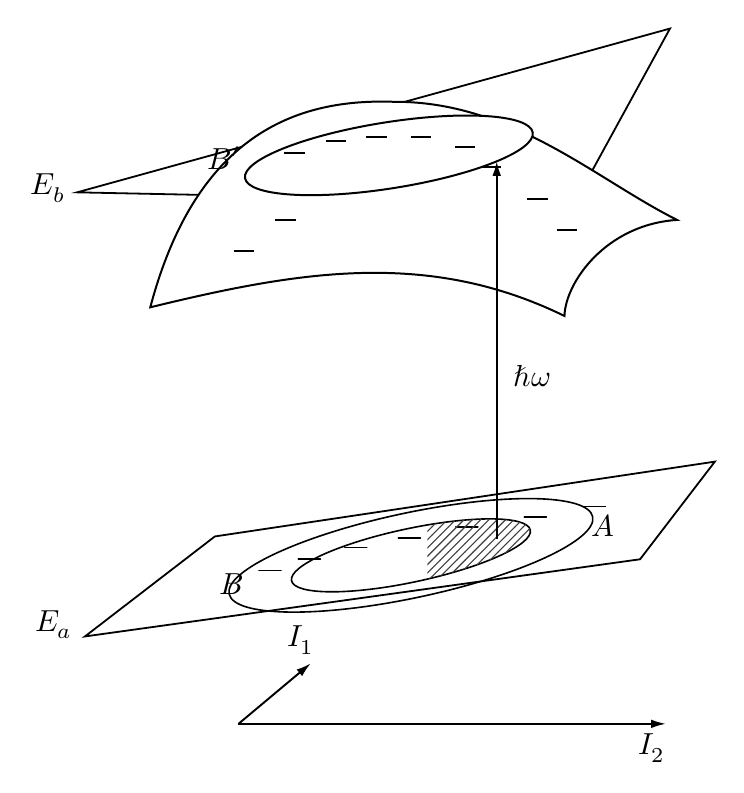
\begin{tikzpicture}[x=1cm,y=1cm]
% Lower resonant energy surface and its oblique reference plane.
\path[draw=black,line width=.65pt,fill=white]
 (.40,1.39)--(7.45,2.37)--(8.40,3.61)--(2.05,2.66)--cycle;
\node[txt,anchor=east] at (.29,1.54) {$E_a$};
% Dashed local levels in the plane, exposed only inside the lower projected section.
\foreach \x/\y in {2.75/2.23,3.25/2.37,3.84/2.52,4.52/2.64,5.25/2.78,6.12/2.91,6.87/3.04}{
 \draw[fine] (\x-.14,\y)--(\x+.14,\y);}
% Large outer oval, inner resonant oval; both are separate geometric contours.
\draw[fine,rotate around={12:(4.54,2.42)}] (4.54,2.42) ellipse (2.36 and .54);
\draw[fine,rotate around={12:(4.54,2.42)}] (4.54,2.42) ellipse (1.55 and .34);
\begin{scope}
 \clip[rotate around={12:(4.54,2.42)}] (4.54,2.42) ellipse (1.55 and .34);
 \fill[pattern=north east lines,pattern color=black!75] (4.75,1.80) rectangle (7.25,3.18);
\end{scope}
\node[txt] at (6.98,2.80) {$A$};
\node[txt] at (2.25,2.06) {$B$};
% Upper reference plane stays behind the curved sheet.
\path[draw=black,line width=.65pt,fill=white]
 (.30,7.03)--(7.83,9.11)--(6.62,6.90)--cycle;
\node[txt,anchor=east] at (.20,7.08) {$E_b$};
% Rear and front branches of the bent upper energy surface.
% Draw as distinct curves so no fictitious plane-plane intersections are created.
\path[draw=black,line width=.72pt,fill=white]
 (1.23,5.57) .. controls (1.83,7.83) and (3.16,8.22) .. (4.32,8.18)
 .. controls (5.82,8.19) and (6.88,7.20) .. (7.92,6.68)
 .. controls (7.01,6.62) and (6.50,5.88) .. (6.49,5.46)
 .. controls (4.77,6.30) and (3.15,6.04) .. (1.23,5.57)--cycle;
% Sparse energy marks drawn on the upper branch only.
\foreach \x/\y in {2.42/6.29,2.95/6.68,3.58/7.11,4.21/7.44,4.92/7.55,5.56/7.35,6.15/6.94,6.52/6.55}{
 \draw[line width=.72pt] (\x-.13,\y)--(\x+.13,\y);}
% Upper elliptical zone, carrying another independent set of levels.
\path[draw=black,line width=.72pt,fill=white,rotate around={9:(4.26,7.50)}]
 (4.26,7.50) ellipse (1.85 and .42);
\foreach \x/\y in {3.06/7.53,3.59/7.68,4.10/7.73,4.67/7.73,5.23/7.61}{
 \draw[line width=.72pt] (\x-.13,\y)--(\x+.13,\y);}
\node[txt] at (2.18,7.47) {$B'$};
% Vertical laser-induced transition between two actual shell regions.
\draw[arr,line width=.85pt] (5.63,2.63)--(5.63,7.43);
\node[txt,anchor=west,fill=white,inner sep=2pt] at (5.77,4.65) {$\hbar\omega_{\mathrm{л}}$};
% External action-number axes; source I_1 oblique and I_2 horizontal.
\draw[arr] (2.35,.28)--(3.27,1.05);
\node[txt,anchor=south] at (3.14,1.12) {$I_1$};
\draw[arr] (2.35,.28)--(7.78,.28);
\node[txt,anchor=north] at (7.60,.20) {$I_2$};
\end{tikzpicture}
\end{document}
